\chapter{正交性}
本章取$\FF=\RR$，讨论有限维实内积空间；对$\RR^n$使用标准内积$\inp vw=v\tp w$。下文涉及正交性的线性空间均已指定这一正定内积。
\begin{definition}{向量的正交}{vector orthogonal}
	若$\inp vw=0$，则称$v$和$w$正交(orthogonal)，记作$v\perp w$。
\end{definition}
\begin{remark}
	依定义，0和所有向量正交。
\end{remark}
\begin{theorem}{正交的模}{}
	若向量$v\perp w$，则
	\begin{align}
		\norm v^2+\norm w^2=\norm{v+w}^2.
	\end{align}
\end{theorem}

\section{正交性}

\begin{definition}
	{向量和子空间的正交}{}
	给定线性空间$L$及其子空间$W$，给定$v\in L$，若$\forall w\in W$均有$v\perp w$，则称$v$和$W$正交，记作$v\perp W$。
\end{definition}

\begin{definition}{子空间的正交}{subspace orthogonal}
	给定线性空间$L$的两个子空间$V,W$，若$\forall v\in V,w\in W$均有$v\perp w$，则称$V$和$W$正交，记作$V\perp W$。
\end{definition}
\begin{corollary}
	若$L$的子空间$V,W$正交，则
	\begin{align}
		\dim(L)\geqslant\dim(V)+\dim(W).
	\end{align}
\end{corollary}
\begin{definition}{正交补}{orthogonal complement}
	线性空间$L$的子空间$V$的正交补(orthogonal complement)由$L$中所有同$V$正交的向量组成，记作$V^\perp$。
\end{definition}
\begin{corollary}
	$V\cap V^\perp=\{0\}$。
\end{corollary}
\begin{theorem}{线性代数基本定理·二}{fundamental theorems of linear algebra II}
	在$\FF^n$中，$\N(A)=\C(A\tp)^\perp.$

	在$\FF^m$中，$\N(A\tp)=\C(A)^\perp.$
\end{theorem}
\begin{theorem}{分解}{resolve}
给定矩阵$A\in\FF^{m\times n}$，则$\forall x\in\FF^n$均可以分解成
\[
	x=x_\mathrm r+x_\mathrm n,
\]
其中$x_\mathrm r\in\C(A\tp),\enspace x_\mathrm n\in\N(A)$，且这种分解是唯一的。
\end{theorem}
\begin{proof}
	由正交性，$\C(A\tp)\cap\N(A)=\{0\}$；又由线性代数基本定理，
	\[
		\dim\C(A\tp)+\dim\N(A)=\rank(A)+n-\rank(A)=n.
	\]
	因此这两个子空间的基合起来构成$\RR^n$的一组基，保证每个$x$都有上述分解。若存在两种分解，则两者的行空间分量之差也在零空间中，只能为零，故分解唯一。
\end{proof}
\begin{theorem}
	{矩阵的可逆部分}{}
	设$\rank(A)=r$。限制映射$A:\C(A\tp)\to\C(A)$是双射；在这两个$r$维空间中分别选基，其表示矩阵为$r$阶可逆矩阵。这里需要先按这四个子空间选择坐标基，不能把零空间理解为原矩阵中可以直接删除的若干行或列。
\end{theorem}
\begin{center}
    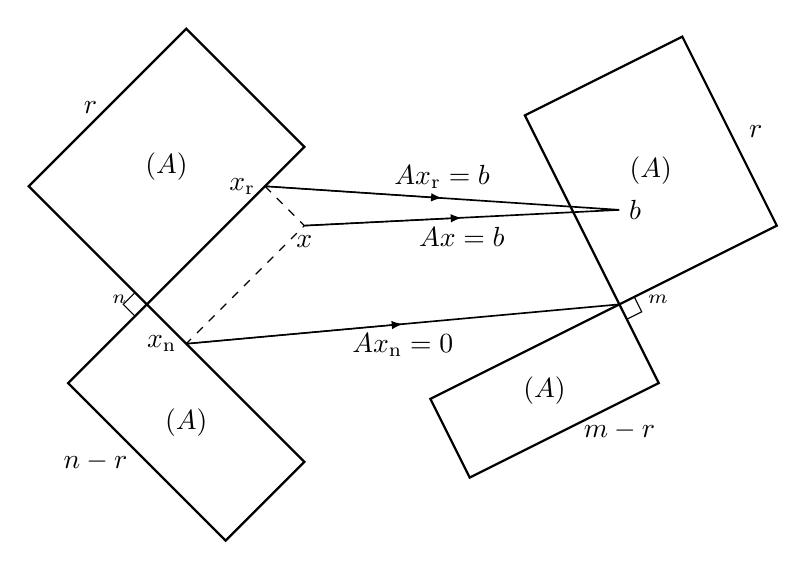
\begin{tikzpicture}
        \draw[thick](0, 0)node[left]{$\RR^n~$}--(2, 2)--(.5, 3.5)--(-1.5, 1.5)node[midway, left]{$r$}--(2, -2)--(1, -3)--(-1, -1)node[midway, left]{$n-r~$}--cycle;
        \draw(-.15, .15)--(-.3, 0)--(-.15, -.15);
        \node at(.25, 1.75){$\C(A\tp)$};
        \node at(.5, -1.5){$\N(A)$};
        \draw[thick](6, 0)node[right]{$~~\RR^m$}--(8, 1)--(6.8, 3.4)node[midway, right]{$~r$}--(4.8, 2.4)--(6.5, -1)--(4.1, -2.2)node[midway, right]{$~m-r$}--(3.6, -1.2)--cycle; % +6
        \draw(6.19, .095)--(6.285, -.095)--(6.095, -.19); % .03√10
        \node at(6.4, 1.7){$\C(A)$};
        \node at(5.05, -1.1){$\N(A\tp)$};
        \coordinate[label=below:$x$](X)at(2, 1);
        \coordinate[label=left:$x_\mathrm r$](R)at(1.5, 1.5);
        \coordinate[label=left:$x_\mathrm n$](N)at(.5, -.5);
        \coordinate[label=right:$b$](B)at(6, 1.2);
        \draw[dashed](R)--(X)--(N);
        \draw[semithick](R)--(B)--(X);
        \draw[semithick](N)--(6, 0);
        \draw[-latex](R)--(3.75, 1.35)node[above]{$Ax_\mathrm r=b$};
        \draw[-latex](X)--(4, 1.1)node[below]{$Ax=b$};
        \draw[-latex](N)--(3.25, -.25)node[below]{$Ax_\mathrm n=0$};
    \end{tikzpicture}
    \captionof{figure}{big picture升级版}
\end{center}
\section{投影}
\begin{example}
	{向量在向量上的投影}{}
	考虑向量$b$在非零向量$a$所张成的直线上的投影(projection)~$p$，依内积的性质：
	\[
		p=(\hat a\cdot b)\hat a=\frac{a\tp b}{a\tp a}a=\frac{aa\tp}{a\tp a}b.
	\]
	那么对于一个矩阵，投影的概念应该如何定义？
\end{example}

考虑$\RR^m$中$n$个线性无关的向量$a_1,\ldots,a_n$张成的子空间$\lspan(a_1,\ldots,a_n)=\C(A)$，其中$A=[a_1\enspace\cdots\enspace a_n]$。向量$b\in\RR^m$在$\C(A)$上的投影为$p\in\C(A)$
\[
	p=Ax=x_1a_1+\cdots+x_na_n.
\]
投影的性质要求：$p$的终点在$\C(A)$中，且距离$b$的终点最近，即$(b-p)\perp\C(A)$，等价于
\[
	A\tp(b-Ax)=0,
\]
相当于求解线性方程组
\[
	A\tp Ax=A\tp b.
\]
若$A\tp A$可逆，则$x=(A\tp A)\iv A\tp b$，故$b$在$\C(A)$上的投影为$p=Ax=A(A\tp A)\iv A\tp b$。
\begin{definition}
	{投影矩阵}{projection matrix}
	对列满秩矩阵$A\in\RR^{m\times n}$，其列空间的正交投影矩阵(orthogonal projection matrix)为
	\begin{align}
		P=A(A\tp A)\iv A\tp.
	\end{align}
\end{definition}

\begin{corollary}
	$P^2=P$且$P\tp=P$。幂等性表示重复投影不改变结果；对称性保证投影方向与目标子空间正交。仅有$P^2=P$也可能是斜投影。
\end{corollary}

\begin{remark}
	只有当$A$可逆时，才能拆开$(A\tp A)\iv=A\iv(A\tp)\iv$，此时$P=AA\iv(A\tp)\iv A\tp=I$。
\end{remark}

\begin{theorem}{$A\tp A$的可逆性}{ATA inverse}
	$A\tp A$可逆$\iff A$的列之间线性无关。
\end{theorem}
\begin{proof}
	只需证明$\N(A\tp A)=\N(A)$即可。
	
	一方面：$\forall x\in\N(A)$，对$Ax=0$左乘$A\tp$得$A\tp Ax=0$，故$x\in\N(A\tp A)$；
	
	另一方面：$\forall x\in\N(A\tp A)$，对$A\tp Ax=0$左乘$x\tp$得
	\[
		x\tp A\tp Ax=\norm{Ax}^2=0\implies Ax=0\implies x\in\N(A).
	\]
	综上，$\N(A\tp A)=\N(A)$。
\end{proof}
\begin{corollary}
	\[
		\rank(A)=\rank(A\tp)=\rank(A\tp A)=\rank(AA\tp).
	\]
\end{corollary}

\section{最小二乘法}

\paragraph{问题背景}
考虑$A\in\RR^{m\times n}$和$b\in\RR^m$。当$m>n$时，方程组可能无精确解，但是否有解仍取决于$b\in\C(A)$，不能单靠矩阵形状判断。无论是否相容，都可寻找使$\norm{b-Ax}$最小的最小二乘解$x'$：
\[
	x'\in\arg\min_x\norm{b-Ax},
\]
由投影的性质，$Ax'$是$b$在$\C(A)$上的唯一正交投影，所有最小二乘解均满足正规方程
\[
 A\tp Ax'=A\tp b.
\]
当且仅当$A$列满秩时，系数向量$x'$唯一，此时
\begin{equation}
	x'=(A\tp A)\iv A\tp b.
\end{equation}
若$A$列不满秩，拟合向量$Ax'$仍唯一，但系数$x'$可加上任意$\N(A)$中的向量。以下拟合公式均须先检查列满秩条件。

\begin{example}{直线拟合(最小二乘法)}{least square}
	$m$组数据$(x_i,y_i)$，确定线性关系$y=a+bx$中的系数$a,b$，即 
	\[
		\begin{bmatrix}
			1&x_1\\\vdots&\vdots\\1&x_m
		\end{bmatrix}
		\begin{bmatrix}
			a\\b
		\end{bmatrix}=
		\begin{bmatrix}
			y_1\\\vdots\\y_m
		\end{bmatrix}\iff Ax=b.
	\]
	\newcommand*{\sumi}[1]{\langle{#1}\rangle}
	若$m\geq2$且$x_i$不全相同，则$A$列满秩$\rank(A)=2$，从而$A\tp A$可逆；否则截距与斜率不能分别确定。满足满秩条件时，
	\[
		A\tp A=
		\begin{bmatrix}
			m&\sumi{x_i}\\
			\sumi{x_i}&\sumi{x_i^2}
		\end{bmatrix},\quad
		(A\tp A)\iv=\frac1{m\sumi{x_i^2}-\sumi{x_i}^2}
		\begin{bmatrix}
			\sumi{x_i^2}&-\sumi{x_i}\\
			-\sumi{x_i}&m
		\end{bmatrix}.
	\]
	为了简化符号，此处且仅在此处$\sumi{\cdot}$特指对$i=1,\ldots,m$求和，得到 
	\begin{equation}
		\begin{cases}
			a=\frac{\sumi{x_i^2}\sumi{y_i}-\sumi{x_i}\sumi{x_iy_i}}{m\sumi{x_i^2}-\sumi{x_i}^2}\\[2ex]
			b=\frac{-\sumi{x_i}\sumi{y_i}+m\sumi{x_iy_i}}{m\sumi{x_i^2}-\sumi{x_i}^2}
		\end{cases}
	\end{equation}
	\iffalse
	\[
		A\tp A=
		\begin{bmatrix}
			n&\textstyle\sum_{i=1}^n x_i\\
			\textstyle\sum_{i=1}^n x_i&\textstyle\sum_{i=1}^n x_i^2
		\end{bmatrix}
	\]
	则
	\[
		(A\tp A)\iv=\frac1{\textstyle{n\sum_{i=1}^n x_i^2-\bigp{\sum_{i=1}^n x_i}^2}}
		\begin{bmatrix}
			\textstyle\sum_{i=1}^n x_i^2&-\textstyle\sum_{i=1}^n x_i\\
			-\textstyle\sum_{i=1}^n x_i&n
		\end{bmatrix}
	\]
	得到 
	\[
		\begin{cases}
			a=\frac{\textstyle\sum_{i=1}^n x_i^2\sum_{i=1}^n y_i-\sum_{i=1}^n x_i\sum_{i=1}^n x_iy_i}{\textstyle{n\sum_{i=1}^n x_i^2-\bigp{\sum_{i=1}^n x_i}^2}}\\[2ex]
			b=\frac{\textstyle-\sum_{i=1}^n x_i\sum_{i=1}^n y_i+n\sum_{i=1}^n x_iy_i}{\textstyle{n\sum_{i=1}^n x_i^2-\bigp{\sum_{i=1}^n x_i}^2}}
		\end{cases}
	\]
	\fi
\end{example}
\begin{example}{多项式拟合}{}
	$m$组数据$(x_i,y_i)$，使用$n$次多项式拟合：
	\[
		y=a_0+a_1x+\cdots+a_nx^n,
	\]
	求$n+1$个系数$a_0,\ldots,a_n$，即 
	\[
		\begin{bmatrix}
			1&x_1&\cdots&x_1^n\\\vdots&\vdots&\ddots&\vdots\\1&x_m&\cdots&x_m^n
		\end{bmatrix}
		\begin{bmatrix}
			a_0\\\vdots\\a_n
		\end{bmatrix}=
		\begin{bmatrix}
			y_1\\\vdots\\y_m
		\end{bmatrix}\iff Ax=b.
	\]
	当采样点中至少有$n+1$个互不相同的$x_i$时，$A$列满秩，从而系数唯一且$x'=(A\tp A)\iv A\tp b$；若不满足此条件，则系数不唯一。
	% \[
	% 	A_{ij}=x_i^{j-1},\quad(A\tp A)_{ij}=\sum_{k=1}^nx_k^{i+j-2}.
	% \]
\end{example}
% 一般最小二乘拟合：……

\begin{remark}
	两组数据相关不一定代表有因果。
\end{remark}

\section{正交归一基}

基是一组线性无关的向量并且张成整个线性空间，我们对基之间的夹角和长度并没有要求。为了方便，我们可以要求基具备一些额外的性质。
\begin{definition}{正交归一基}{orthonomal basis}
	$n$维线性空间中的一组基$\{q_1,\ldots,q_n\}$若满足， 
	\[
		\inp{q_i}{q_j}=\delta_{ij},\quad\forall i,j.
	\]
	则称这组基是正交归一的(orthonomal)。
\end{definition}

\begin{definition}
	{正交矩阵}{orthogonal matrix}
	将$\RR^n$的一组正交归一基$\{q_1,\ldots,q_n\}$按列排成矩阵
	\[
		Q=[q_1\enspace\cdots\enspace q_n],
	\]
	则$Q$是方阵且$Q\tp=Q\iv$，称$Q$为正交矩阵(orthogonal matrix)。
\end{definition}
\begin{theorem}
	{正交归一基的完备性}{completeness}
	由$Q\tp Q=QQ\tp=I$，可得正交归一基的完备性(completeness)
	\begin{equation}
		\sum_{i=1}^nq_iq_i\tp=I.
	\end{equation}
\end{theorem}
% \begin{example}{Fourier级数}{Fourier series}
% 	定义函数$f,g$在$[-\pi,\pi]$上的内积
% 	\[
% 		\inp fg:=\int_{-\pi}^\pi f(x)g(x)\d x,
% 	\]
% 	则三角函数系列
	% \[
	% 	\biggB{\frac1{\sqrt{2\pi}},\frac{\sin\theta}{\sqrt\pi},\frac{\cos\theta}{\sqrt\pi},\frac{\sin2\theta}{\sqrt\pi},\frac{\cos2\theta}{\sqrt\pi},\ldots},
	% \]
% 	构成一组正交归一基，任意$[-\pi,\pi]$上平方可积的函数$f(x)$均可被展开为Fourier级数(Fourier series)：
% 	\[
% 		f(x)=\frac{a_0}2+\sum_{n=1}^\infty(a_n\cos nx+b_n\sin nx),
% 	\]
% 	其中Fourier系数
% 	\[
% 		\begin{cases}
% 			a_n:=\frac1\pi\int_{-\pi}^\pi f(x)\cos nx\d x,\\[2ex]
% 			b_n:=\frac1\pi\int_{-\pi}^\pi f(x)\sin nx\d x.
% 		\end{cases}
% 	\]
% \end{example}

\subsection{Gram-Schmidt法则}

给定一组基$\{a_1,\ldots,a_n\}$，如何构造一组正交归一基？

\begin{method}{Gram-Schmidt法则}{Gram-Schmidt rule}
	\begin{compactenum}
		\item 选取$b_1:=a_1;$
		% \item 从$a_2$减去沿着$b_1$方向的分量，作为$b_2$
		% \[
		% 	b_2:=a_2-\frac{\inp{b_1}{a_2}}{\inp{b_1}{b_1}}b_1;
		% \]
		\item 从$a_i$减去沿着$b_1,\ldots,b_{i-1}$方向的分量，作为$b_i$
		\[
			b_i:=a_i-\sum_{j=1}^{i-1}\frac{\inp{b_j}{a_i}}{\inp{b_j}{b_j}}b_j.
		\]
	\end{compactenum}
	因为输入向量线性无关，每个$b_i$都非零。得到正交基$\{b_1,\ldots,b_n\}$后，再归一化$q_i=\hat b_i$，便得到正交归一基。若输入只是生成集而非基，则可能出现$b_i=0$；此时应跳过该向量，不能除以其范数。
\end{method}

\subsection{\texorpdfstring{$QR$}{QR}分解}

\begin{theorem}{QR分解}{QR decomposition}
	若$m\times n$矩阵$A=(a_1,\ldots,a_n)$的列之间线性无关，可用Gram-Schmidt法则构造一组正交归一基$\{q_1,\ldots,q_n\}$，$q_i$同$a_1,\ldots,a_{i-1}$正交，定义
	\[
		R:=Q\tp A=\begin{bmatrix}
			q_1\tp a_1&q_1\tp a_2&\cdots&q_1\tp a_n\\[1ex]
			&q_2\tp a_2&\cdots&q_2\tp a_n\\
			&&\ddots&\vdots\\
			&&&q_n\tp a_n
		\end{bmatrix}
	\]
	$Q=[q_1\enspace\cdots\enspace q_n]\in\RR^{m\times n}$满足$Q\tp Q=I_n$，$R\in\RR^{n\times n}$是对角元非零的上三角矩阵，且$\C(Q)=\C(A)$，故
	\begin{equation}
		A=QR.
	\end{equation}
	这称为薄QR分解。当$m>n$时，$Q$不是正交方阵，$QQ\tp$是$\C(A)$上的投影；仅当$m=n$时才有$QQ\tp=I_m$及$Q\tp=Q\iv$。
\end{theorem}

\begin{remark}
	在最小二乘法等应用中，$A\tp A=R\tp R$
	\[
		x=(A\tp A)\iv A\tp b=R\iv Q\tp b.
	\]
	计算时通过回代求解$Rx=Q\tp b$，不必显式形成$R\iv$或$A\tp A$。
\end{remark}
